\chapter{Hardware attacks taxonomy}
First of all, we must define what it is an hardware attack.
\begin{boxH}
  An \textbf{hardware attack} is the act of exploiting a vulnerability in the hardware to perform an
  attack.
\end{boxH}
All hardware design don't cover all the possibilities, because in some cases the risk is accepted,
so there's always a surface of attack. Those can be classified according to:
\begin{itemize}
  \item Their goal (stealing, corrupting or inhibiting)
  \item Their target (information or property)
  \item Their modality (invasive or non-invasive)
  \item Their domain (logical or physical).
\end{itemize}

\begin{figure}[H]
  \centering
  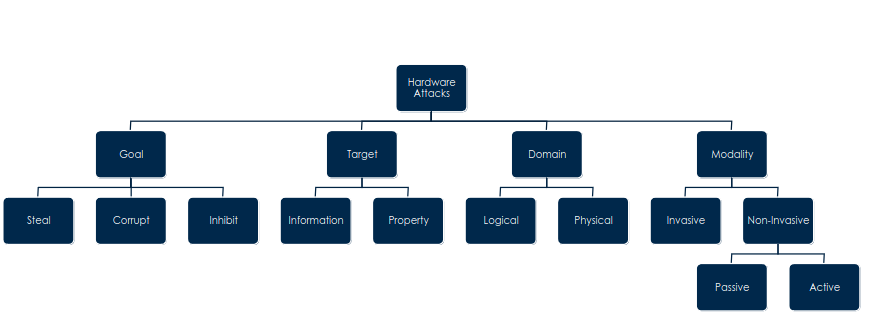
\includegraphics[width=0.8\textwidth]{img/hardware/hw attacks taxonomy.png}
  \caption{Hardware attacks taxonomy}
  \label{fig:hw-attacks-taxonomy}
\end{figure}

An attack exploits a vulnerability that harms one of the three CIA properties: confidentiality,
integrity and availability. The goal of the attack can be stealing, corrupting the target(memory
words, permission from files, etc.) or inhibiting the target (a service, a set of critical data, etc.).
The point of most of the attacks is not to be stealthy, but to be effective.\\
The \textbf{target} of a hardware attack is always \textbf{an asset} treated or owned by a hardware
component, which can be:
\begin{itemize}
  \item A piece of information treated by the hardware (a key, some credentials, a protected memory word
    or file, etc.)
  \item A property owned by the hardware (its IP, one of its resources or functionalities, etc.)
\end{itemize}

Those attacks can be carried out in two way:
\begin{itemize}
  \item in a \textbf{logical} way, exploding the hardware from the software
  \item in a \textbf{physical} way, exploiting the hardware vulnerability in a direct fashion
\end{itemize}

The attacks also differs in the modality in which are carried out:
\begin{itemize}
  \item \textbf{Invasive attacks}, Require actions against the attacked hardware (e.g., desoldering,
    repackaging, disconnections) to allow physical intrusions to access some internal components
    easily. Those attacks leave physical traces.
  \item \textbf{Non-invasive attacks}, which can be carried out without the physical access to the
    hardware, and are further divided into:
    \begin{itemize}
      \item \textbf{passive} non-invasive attacks, carried out by analyzing and measuring one (or
        more) physical dynamic entities of the attacked hardware
      \item \textbf{active} non-invasive attacks, which require specific actions on the device to
        force the system into abnormal states, in which the attacker’s goal is easier to reach.
    \end{itemize}
\end{itemize}
Those attacks usually require moderate investment in therms of lab equipment and effort in the
design of the attack on the target device.
\begin{figure}[H]
  \centering
  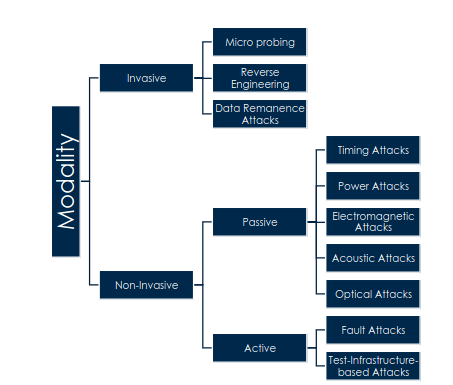
\includegraphics[width=0.6\textwidth]{img/hardware/hw attacks modalities.png}
  \caption{Some examples of hw attacks}
  \label{fig:hw-attacks-modality}
\end{figure}
